%\animategraphics[autoplay,loop,width=5cm,controls=all]{30}{Fotos/Vacío/gif/foo-}{0}{77}
\section{Introducción}
    \subsection{Objetivos}
        En este breve informe descubriremos y analizaremos el comportamiento del líquido más abundante de nuestro planeta (el agua) cuando es sometido a presiones inferiores a la atmosférica. Usaremos nuestros conocimientos, además de los contenidos vistos en las clases de laboratorio, para lograr describir el comportamiento del agua.
    \subsection{Descripción de la experiencia}
        La experiencia de laboratorio se basa en cuatro elementos, un vaso, un termómetro, cámara de vacío y un bomba de aire.\\ \\
        El primer paso es llenar nuestro vaso con agua del grifo normal, y colocar un termómetro en su interior. Observamos como el agua se encuentra a unos $2\si{celsius}$ por debajo de la temperatura ambiente. Seguidamente, introducimos dicho vaso en nuestra cámara de vacío, que consiste en una base circular con una goma en el borde sobre la cual ponemos una cúpula transparente. Hemos de fijarnos en la posición del termómetro dentro de la cámara, para que podamos realizar mediciones mientras la cámara está cerrada. \\ \\ Como último paso, encendemos el motor de la bomba de aire y abrimos la válvula que la comunica con la cámara de vacío. Mientras la presión va disminuyendo dentro de la cámara observamos cómo en el agua empiezan a formarse burbujas. Finalmente, una vez el motor alcanza el máximo de presión que puede mantener (alrededor de $-0.8\textit{atm}$), vemos como el agua hierve, pero sin haber aumentado su temperatura respecto a la ambiente.\\ \\Hay que recalcar que no solo es que la temperatura del agua no haya aumentado, si no que va disminuyendo lentamente.
\section{Propuesta de Hipótesis}
    Lo más destacable de la experiencia es que resulta chocante ver agua hervir a temperatura ambiente. Estamos acostumbrados a hervir agua en el fuego y tomamos por hecho que el agua hierve a $100\si{\celsius}$, sin tener en cuenta que esta medida es a $1\textit{attm}$ de presión, y si variamos la presión variaremos el punto de ebullición del agua. Es bien sabido que el cambio de fase del agua depende tanto de la temperatura como de la presión, pero nuestra primera impresión lo ignora.\\ \\Podemos explicar este comportamiento con un diagrama de los cambios de fase del agua. Como vemos en la figura \ref{fig:fase}, a unos $25\si{\celsius}$, cuando disminuimos la presión (eje $y$) sucede un cambio de fase de agua líquida a vapor.\\
    \begin{figure}[h]\label{fig:fase}
        \centering
        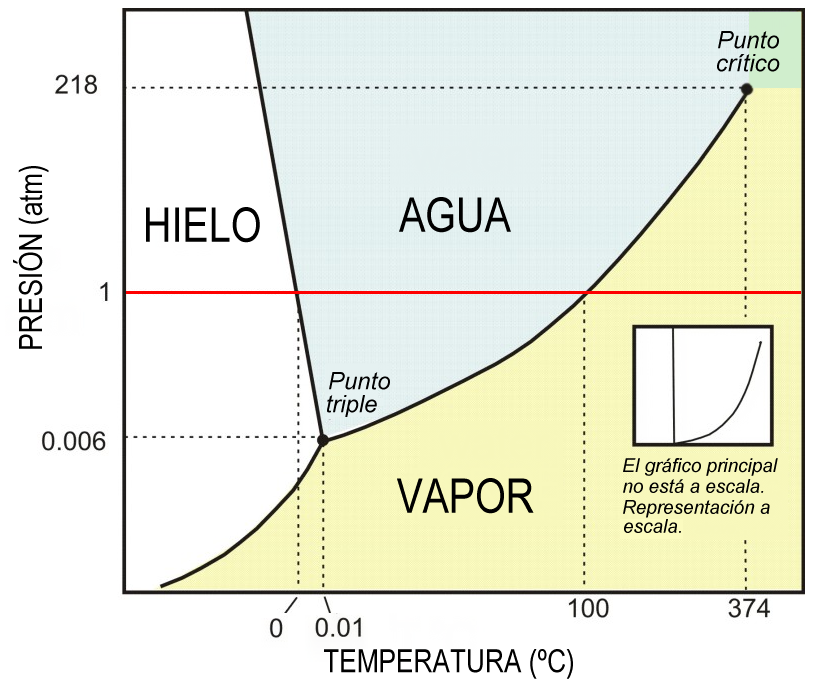
\includegraphics[width=.55\textwidth]{Fotos/Vacío/fase.png}
        \caption{Diagrama de fase del agua}
    \end{figure}
    \hfill{}\\
    Además, al cambiar de fase, el agua disipa energía al hervir, lo que explica la disminución de temperatura que observamos experimentalmente.
\section{Comprobación y discusión}
    Es bien sabido que los alpinistas que escalan los grandes picos de nuestro planeta requieren de una gran capacidad pulmonar. Esto no es solo por el gran esfuerzo físico que sus hitos requieren, si no porque la concentración de oxígeno es menor cuanto mayor es la altitud. Pero esta no es la única consecuencia de la gran altitud a la que los deportistas se ven sometidos, también existe una disminución en la presión atmosférica.\\ \\Cuanto más altura tomemos, menor es la columna de aire que tenemos sobre nuestras cabezas, es decir, la presión atmosférica sobre nosotros disminuye. Y es que el punto de ebullición del agua a la altura del Mt. Everest es de tan solo $70\si{\celsius}$. Extrapolándolo a nuestro experimento, si siguiéramos subiendo más allá de la altura del Everest, sería equivalente a disminuir la presión en nuestra cámara.\\ \\También es por esto que los aviones han de ser presurizados para subir a las altitudes operativas, el cuerpo humano está compuesto por agua al fin y al cabo, y hervir literalmente la sangre de los pasajeros no es una buena estrategia comercial.

\section{Sugerencias experimentales}
    La sugerencia más clara que puedo comentar, es que una bomba de vacío con mayor potencia (y un equipo acorde, válvulas con menores pérdidas de aire etc.) mejoraría la experiencia. Y es que dicho equipo no solo haría hervir el agua más violentamente, sino que haría disminuir la temperatura del agua con mayor velocidad.\\ \\No es el objetivo de este informe, pero esto daría pie a preguntarnos qué pasaría si dejáramos el agua hervir por ejemplo, media hora, con el consecuente descenso en la temperatura. Con una cámara que mantuviera esta presión cercana a $-1\textit{atm}$ la temperatura del agua podría rondar los $0\si{\celsius}$ y dar lugar a la cuestión de si el agua se congelaría o continuaría hirviendo. Podemos encontrar evidencias de que el agua se congelaría en internet (ver referencia \ref{video}), pero es un marco de estudio sobre el que se podría profundizar\\ \\Esta cuestión podría dar lugar a un informe de mayor profundidad sobre el tema, que resultaría todavía más atractivo e impresionante de presentar (¡Agua hirviendo que se congela!).
\section{Referencias}
    \hyperlink{https://www.youtube.com/watch?v=y4BGV7-1lhs&t=7s}{YouTube - Boiling Water Until It Freezes, por Cody'sLab}\label{video}\\ \\
    \hyperlink{https://www.liceoagb.es/quimigen/liqu7.html}{liceoagb.es - Líquidos y sólidos, diagramas de fase}